\documentclass[assd_tp3_main.tex]{subfiles}

\begin{document}

\section{Modulador delta}

El segundo conversor anal\'ogico/digital que se implement\'o fue un modulador delta. El mismo hace uso del principio de que, al muestrear una se\~nal a una frecuencia mucho mayor a la de Nyquist (oversampling), el valor de la misma no se altera significativamente entre muestra y muestra. Por lo tanto, codificando la diferencia entre una muestra y la siguiente, en lugar del valor de la muestra en s\'i, se puede ganar SQNR sin necesidad de incrementar el n\'umero de bits del ADC. El diagrama de bloques b\'asico de este conversor se observa en la figura \ref{fig:delta-bloques}.

\begin{figure}[htb]
	\centering
	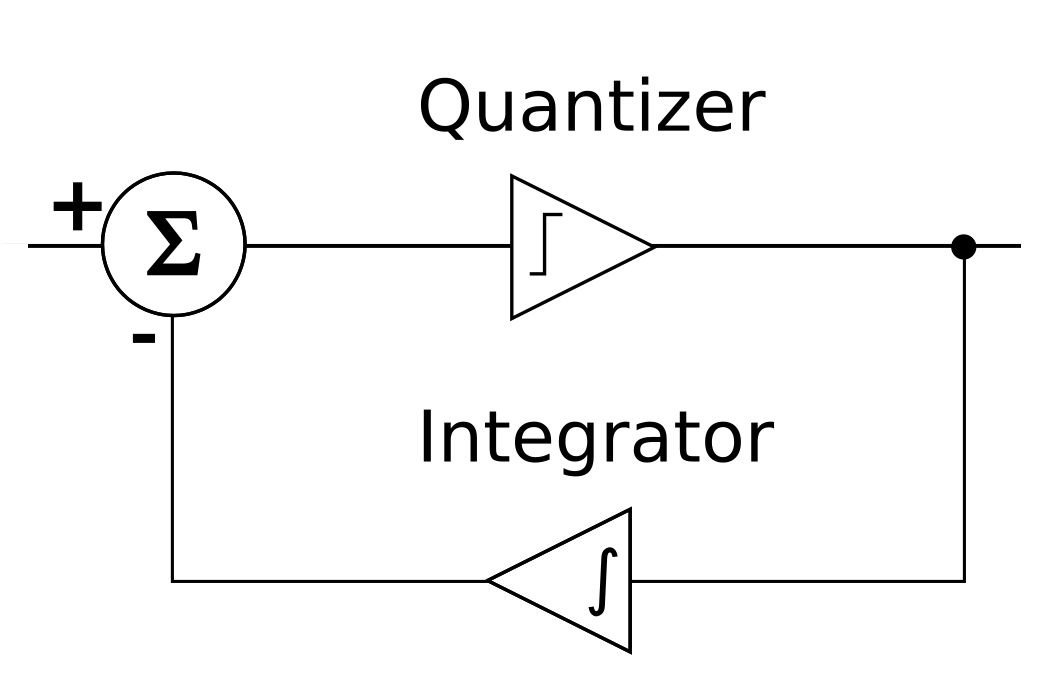
\includegraphics[width=0.6 \textwidth]
	{imagenes/ej3/delta-bloques.png}
	\caption{Diagrama de bloques del modulador delta}
	\label{fig:delta-bloques}
\end{figure}

En este trabajo, la implementaci\'on utiliza la FPGA como integrador y un LM311 para realizar la resta. La FPGA recibe la salida del comparador (que indica si la aproximaci\'on actual es menor o mayor que la entrada), y en funci\'on de la respuesta, incrementa o decrementa un contador de 8 bits. De esta manera, la salida sigue a la entrada en todo momento, si bien hay un tiempo de adquisici\'on proveniente de que la salida solo puede cambiar un LSB por per\'iodo de muestreo.

Este tiempo de adquisici\'on limita la frecuencia m\'axima que se puede seguir con una cierta frecuencia de muestreo $f_s$. Llamamos $\Delta$ a la diferencia entre dos niveles l\'ogicos en la salida (un LSB), que en nuestro caso es:

\begin{equation}
	\Delta = \frac{5\mathrm{V}}{256-1} \sim 0.0196\mathrm{V}
	\label{eq:lsb}
\end{equation}

Luego, la condici\'on para que la salida pueda seguir a la entrada, es decir, que por cada per\'iodo de muestreo $T_s$, la salida no cambie m\'as de 1LSB, queda expresada como:

\[ 
	\frac{dx}{dt} \leq \frac{\Delta}{2T_s}
\]

Si consideramos entradas senoidales de amplitud $V_p$ y frecuencia $f_0$, se obtiene entonces que:

\begin{equation}
	f_s \geq \frac{V_p}{\Delta} \cdot 4\pi f_0
\end{equation}

Considerando el valor obtenido en \ref{eq:lsb}, y que la tensi\'on pico m\'axima es $\nicefrac{5\mathrm{V}}{2} = 2.5\mathrm{V}$, se obtiene que:

\begin{equation}
	f_s \geq 510 \pi \cdot f_0 \simeq 1603 \cdot f_0
\end{equation}


\end{document}